در این فصل به ارائه‌ی برخی کارهای پیشین و مرتبط به موضوع این پژوهش خواهیم پرداخت. در مورد هر یک از این موارد به ارتباط آن با بحث جاری، کاربرد و یا نقاط تأثیرگذار آن در موضوع این پژوهش و هم‌چنین ضعف ها و نقایص آن‌ها پرداخته شده است. 

با توجه به جنبه‌های مختلف این پژوهش، کارهای مرتبط با هر کدام از این جنبه‌ها نیز به طور مستقل مورد بررسی قرار گرفته است. بر این اساس، ساختار این فصل در سه بخش اصلی تنظیم شده است. در بخش \ref{section:iocoTesters} برخی ابزار‌های آزمون خودکار نرم‌افزار که بر مبنای نظریه‌ی آی‌او‌کو رفتار می‌کنند، بررسی می‌شوند. این بررسی‌ها عمدتاً از دو منظر استاندارد و زبان مدل‌سازی و نحوه‌ی ارتباط آزمون‌گر با سیستم تحت آزمون در هر یک از این ابزارها خواهد بود. بخش \ref{section:dataTestTools} برخی از ابزارها و یا روش‌هایی که به طور خاص از داده‌های آزمون پشتیبانی می‌کنند را از نظر خواهد گذراند. در نهایت بخش \ref{section:applications} به توضیح تعدادی از کاربردهای صنعتی استفاده از ابزارهای آزمون مبتنی بر مدل و نتایج به دست آمده از آن خواهد پرداخت. 

\section{الگوهای همگام سازی}
\label{section:coordinationPatterns}
ابزارهای گوناگونی برای آزمون خودکار نرم‌افزار تولید و عرضه شده‌اند که بر پایه‌های مختلف نظری مبتنی هستند. تکیه‌ی ما در این بحث بر روش‌هایی است که از آی‌اوکو به عنوان روش رابطه‌ی مطابقت استفاده می‌کنند. 
\section{طراحی به روش ارتباط ناهمگام}
\label{section:asyncDesign}
این بخش به بررسی روش‌ها و ابزارهایی می‌پردازد که داده‌‌ها را به عنوان ورودی و خروجی سیستم در نظر می‌گیرند و با تولید ترکیب‌های مختلف از مقایر داده‌ای و رد و بدل کردن آن با سیستم به انجام وارسی می‌پردازند.

\subsection{مالتی کور}
بسته‌ی ال‌تی‌جی\LTRfootnote{LEIRIOS Test Generator (LTG)} \cite{Bouquet04LTG} مجموعه‌ی کاملی از ابزارهای آزمون را معرفی می‌کند که هدف آن انجام کلیه‌ی عملیات آزمون از توصیف کارکرد سیستم تا جزئیات داده‌های آن توسط یک ابزار واحد است. ال‌تی‌جی برای مدل‌سازی جنبه‌های مختلف از سه نمادگذاری مختلف پشتیبانی می‌کند. \textit{نمودارحالت یوام‌ال، نمادگذاری بی\LTRfootnote{B Notation} و نمودار کلاس یوام‌ال}. در این ابزار نمودار حالت بیشتر برای توصیف رفتارهای سیستم مورد استفاده قرار می‌گیرد در حالی که توصیف نمادگذاری بی بیشتر برای نمایش ساختارهای داده‌‌ای مورد استفاده قرار می‌گیرد. 

ضابطه‌‌ی انتخاب موارد آزمون در ابزار ال‌تی‌جی بر پایه‌ی معیارهای مختلف برای پوشش\LTRfootnote{coverage} طراحی شده است. برای مثال در مورد نمودارهای حالت یو‌ام‌ال این ابزار از ضابطه‌های پوششی مثل «طی کردن تمام گذارها» و «طی کردن تمام حالت‌ها» پشتیبانی می‌کند. هم‌چنین در آن از موارد توصیف‌های بی ضابطه‌ مانند «پوشاندن تمامی حالت‌های شرط‌ها» پشتیبانی می‌شود.

باید توجه کرد که الگوریتم تولید موارد آزمون در ال‌تی‌جی بر رابطه‌های مطابقت (مانند آی‌او‌کو) متکی نیست بلکه از روش‌های جستجوی فضای حالت و اجرای نمادین محدود شده\LTRfootnote{constraint based symbolic execution} استفاده می‌کند. برای تولید رفتارهای آزمون، آزمون‌گر مسیرهای \emph{مرزی} را در نظر می‌گیرد. به یک مسیر، مرزی اطلاق می‌شود که لااقل یکی از متغیرهای موجود در حالت‌های آن مسیر در حالت کمینه و یا بیشینه قرار داشته باشند. مراحل تولید موارد آزمون در ال‌تی‌جی را می‌توان در سه گام اصلی خلاصه نمود:
\begin{enumerate}
\item تولید حالت‌های مختلف رفتار سیستم با استفاده از مدل رفتاری داده‌شده به سیستم (مانند ماشین‌های حالت)
\item محاسبه‌ی مقادیر داده‌ای به هدف یافتن حالت‌های مرزی به ازای هر یک از رفتارهای سیستم
\item تولید موارد آزمون با استفاده از حالت‌های مرزی و معرفی ترتیب‌هایی از عملیات که در شرط‌های مرزی صدق می‌کنند
\end{enumerate}
شکل \ref{fig:LTGSample}.(الف) نمونه‌ای از توصیف یک ساختار داده‌ای مورد آزمون در نمادگذاری بی را نشان می‌دهد. این مثال می‌تواند توصیف کننده‌ی مدل درختی از رده‌بندی داده‌ باشد که در بخش \ref{section:CategoryPartitionMethod} به آن پرداخته شد. شمای این توصیف درختی در شکل \ref{fig:LTGSample}.(ب) آمده است.
 
\begin{figure*}
    \begin{center}
    \begin{tabular}{| c | c |}
      	\hline
	 & \\
	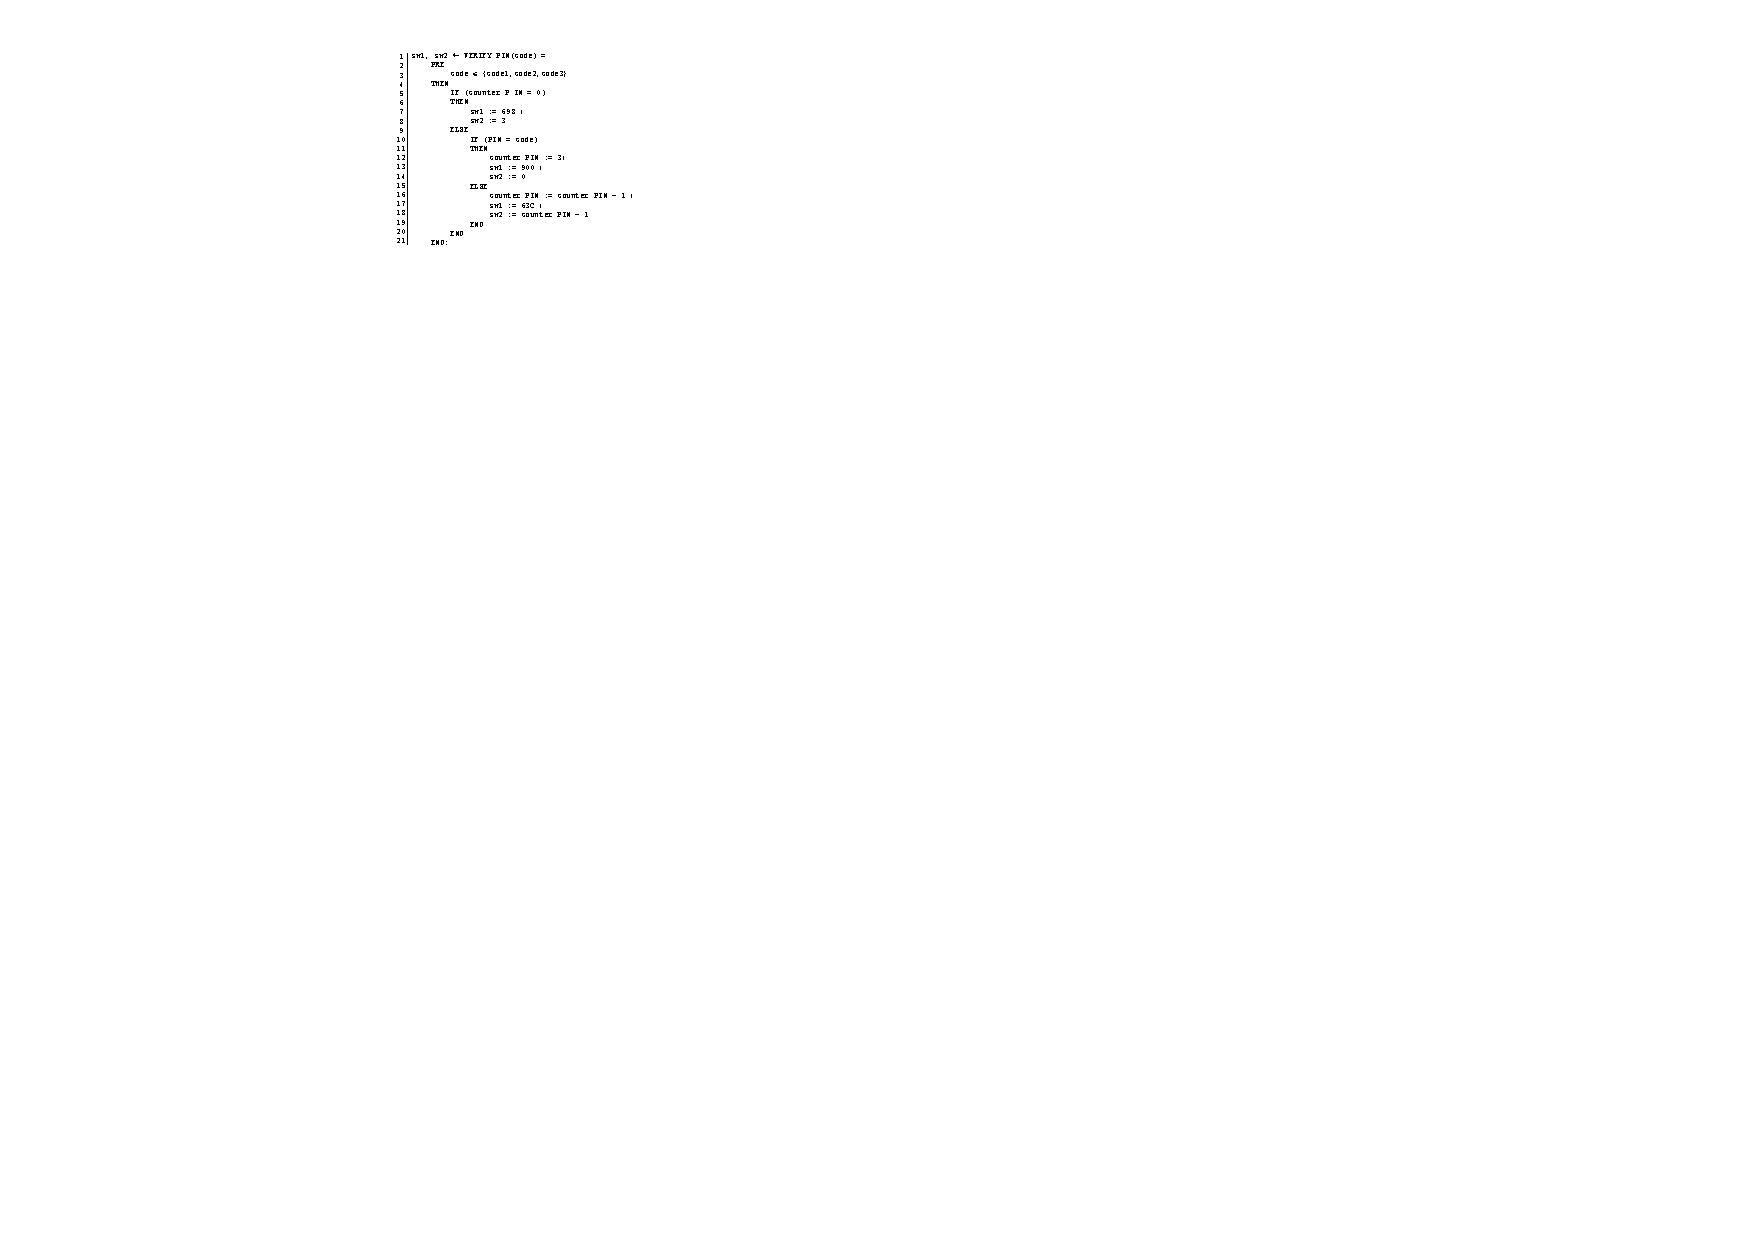
\includegraphics[width=7cm]{3-RelatedWork/Figures/LTGSampleA.pdf} &
         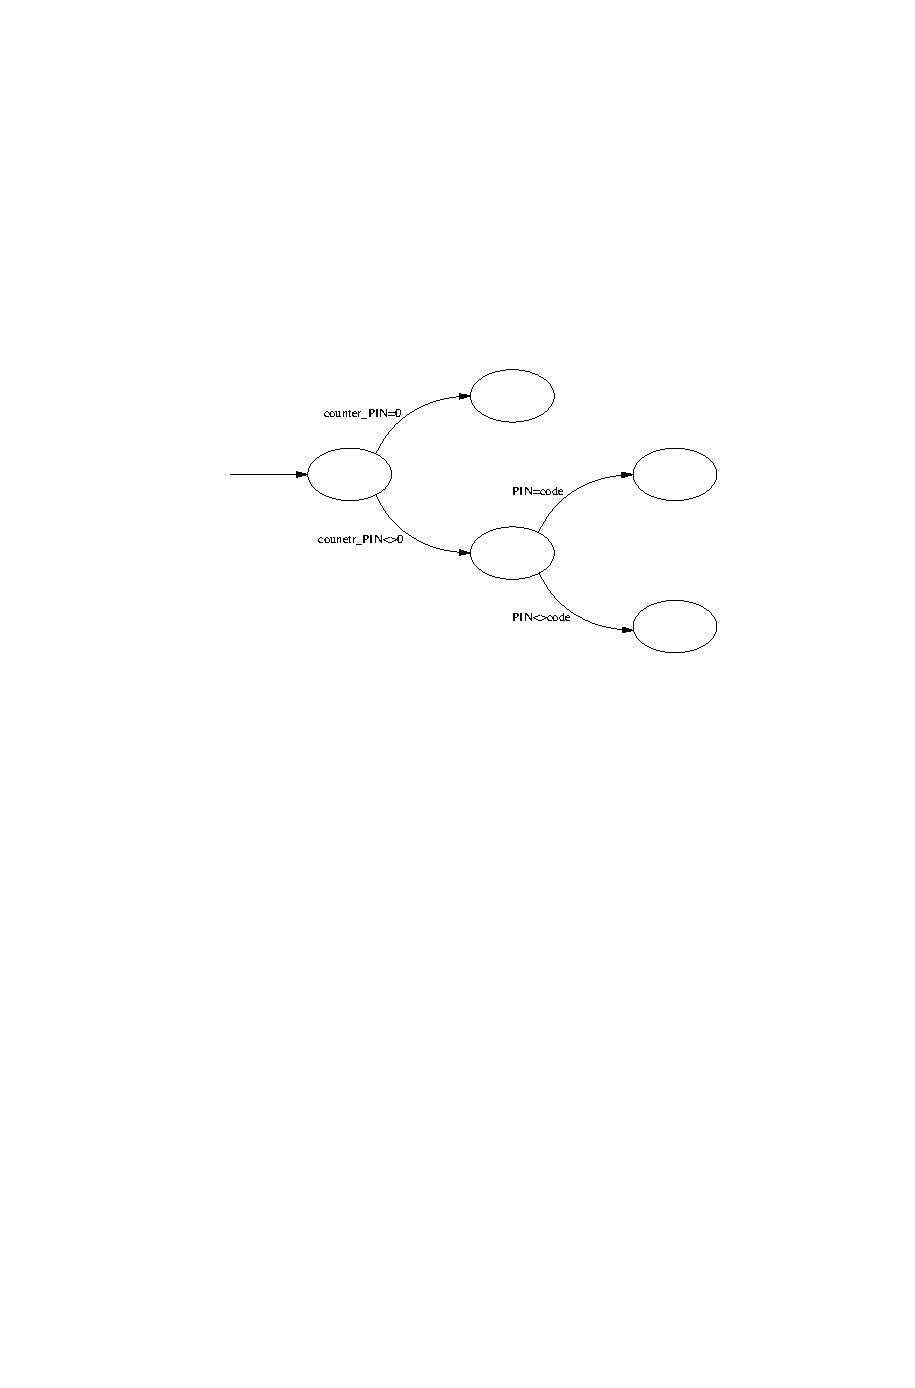
\includegraphics[width=9cm]{3-RelatedWork/Figures/LTGSampleB.pdf} 
 	\\
         (الف) & (ب) \\
	\hline
    \end{tabular}
    \end{center}
    \caption{\label{fig:LTGSample}(الف) نمونه‌ای از یک توصیف ساختار داده‌ای در نمادگذاری بی و (ب) شمای درختی این توصیف}
\end{figure*}

با وجود گستردگی قابلیت‌های آزمون‌گر ال‌تی‌جی، این ابزار محدودیت‌ها و معایب زیادی نیز دارد که در این‌جا به بیان برخی از این موارد می‌پردازیم:
\begin{itemize}
\item آزمون‌گر ال‌تی‌جی اگرچه از تولید خودکار موارد آزمون از روی مدل رفتاری سیستم پشتیبانی می‌کند، اما الگوریتم تولید موارد آزمون در آن مبتنی بر رابطه‌های مطابقت (مانند آی‌اوکو) نیست. نتیجه‌ی عدم پشتیبانی از آی‌اوکو ایجاد محدودیت‌هایی بر روی روش مدل‌سازی است. برای مثال، مدل‌های ورودی ال‌تی‌جی باید همگی متناهی و قطعی باشند در حالی که در آزمون‌گرهایی مانند تورکس چنین محدودیت‌هایی وجود ندارد.
\item علی‌رغم پشتیبانی از مقادیر داده‌ای، در ال‌تی‌جی امکان تعریف و توصیف گونه‌های داده‌ای وجود ندارد. این امر باعث می‌شود که محدودیت‌های زیادی در توصیف انواع گوناگون داده به وجود آید.
\item برای مدل‌سازی جنبه‌های مختلف سیستم در ال‌تی‌جی نیاز به استفاده از نمادگذاری‌های مختلفی است که این امر هم باعث دشواری در نگارش توصیف‌ها و خوانایی و هم دشواری در نگه‌داری مدل‌ها می‌شود.
\item این آزمون‌گر امکان تولید موارد آزمون به صورت در-لحظه را ندارد و موارد آزمون تولید شده باید ابتدا تولید و نگه‌داری شده و سپس برای آزمون سیستم مورد استفاده قرار گیرند.
\end{itemize}

سلام